\chapter{Marco Teórico}

\section{Internet de las Cosas}

La internet de las cosas es un sistema de dispositivos de computación interrelacionados, máquinas mecánicas y digitales, objetos, animales o personas que tienen identificadores únicos y la capacidad de transferir datos a través de una red, sin requerir de interacciones humano a humano o humano a computadora. \\

IoT ha evolucionado desde la convergencia de tecnologías inalámbricas, sistemas micro-electromecánicos, microservicios e internet. La convergencia ha ayudado a derribar las paredes de silos entre la tecnología operativa  y la tecnología de la información, permitiendo que los datos no estructurados generados por máquinas sean analizados para obtener información que impulse mejoras. \cite{TechT2017}\\

Kevin Ashton, cofundador y director ejecutivo del Auto-ID Center de MIT, mencionó por primera vez la internet de las cosas en una presentación que hizo a Procter \& Gamble en 1999. He aquí cómo Ashton explica el potencial de la internet de las cosas:

``Las computadoras de hoy –y, por lo tanto, la internet– dependen casi totalmente de los seres humanos para obtener información. Casi todos los aproximadamente 50 petabytes (un petabyte son 1.024 terabytes) de datos disponibles en internet fueron capturados y creados por seres humanos escribiendo, presionando un botón de grabación, tomando una imagen digital o escaneando un código de barras. \\

El problema es que la gente tiene tiempo, atención y precisión limitados, lo que significa que no son muy buenos para capturar datos sobre cosas en el mundo real. Si tuviéramos computadoras que supieran todo lo que hay que saber acerca de las cosas –utilizando datos que recopilaron sin ninguna ayuda de nosotros– podríamos rastrear y contar todo, y reducir en gran medida los desechos, las pérdidas y el costo. Sabríamos cuándo necesitamos reemplazar, reparar o recordar cosas, y si eran frescas o ya pasadas”. \cite{Asthon2009}\\

\subsection{Plataforma Heroku}

https://www.heroku.com/platform


The Heroku Platform

Heroku is a cloud platform based on a managed container system, with integrated data services and a powerful ecosystem, for deploying and running modern apps. The Heroku developer experience is an app-centric approach for software delivery, integrated with today’s most popular developer tools and workflows.


\subsection{Framework Laravel}

https://web.archive.org/web/20130929055257/http://laravel.com/docs/introduction

https://www.arsys.es/blog/programacion/que-es-laravel/
%Framework del profesor Cesar Alvarez

\subsection{HTTP}

El protocolo de transferencia de hipertexto (HTTP) es un protocolo de la capa de aplicación en el modelo OSI, se usa para transmitir documentos hipermedia, como HTML. Fue diseñado para la comunicación entre navegadores web y servidores web, pero también se puede usar para otros propositos. HTTP sigue un modelo clasico de cliente-servidor, con un cliente que abre una conexión para realizar una petición, luego esperando la respuesta. HTTP es un protocolo sin estado, significa que el servidor no conserva ningun dato entre dos solicitudes. Para realizar las peticiones este protocolo cuenta con diferentes metodos.

%https://developer.mozilla.org/en-US/docs/Web/HTTP

\paragraph{Metodos de solicitud HTTP:}

HTTP define un conjunto de métodos de solicitudes para indicar la acción deseada que se realizará para un recurso determinado. Aunque pueden ser sustantivos, estos métodos algunas veces se denominan verbos HTTP. Cada uno de ellos implementa una semantica diferente, pero algunas caracteristicas comunes son compartidas por un grupo de ellos.\\


\begin{itemize}
	\item GET: este método solicita una representación del recurso especificado. Las peticiones que lo usan, solo deben regresar datos.
	\item HEAD: este método solicita una respuesta igual a una peticion GET, pero sin el cuerpo de la respuesta.
	\item POST: se usa para enviar una entidad al recurso especificado, causando a menudo un cambio en el estado o efectos secundarios en el servidor.
	\item PUT: reemplaza todas las representaciones actuales del recurso destino con la la petición de carga útil.
	\item DELETE: esta petición elimina el recurso especificado.
	\item CONNECT: establece un túnel para el servidor identificado por el recurso de destino.
	\item OPTIONS: se usa para describir las opciones de la comunicación para el recurso destino.
	\item TRACE: realiza una prueba de mensaje loop-back a lo largo de la ruta del recurso de destino. 
	\item PATCH: se usa para realizar modificaciones parciales a un recurso.
\end{itemize}
%The GET method requests a representation of the specified resource. Requests using GET should only retrieve data.

%The HEAD method asks for a response identical to that of a GET request, but without the response body.

%The POST method is used to submit an entity to the specified resource, often causing a change in state or side effects on the server

%The PUT method replaces all current representations of the target resource with the request payload.

%The CONNECT method establishes a tunnel to the server identified by the target resource.

%The OPTIONS method is used to describe the communication options for the target resource.

%The TRACE method performs a message loop-back test along the path to the target resource.

%The PATCH method is used to apply partial modifications to a resource. 

%https://developer.mozilla.org/en-US/docs/Web/HTTP/Methods

\subsection{JSON}

JSON (JavaScript Object Notation - Notación de Objetos de JavaScript) es un formato ligero de intercambio de datos. Leerlo y escribirlo es simple para humanos, mientras que para las máquinas es simple interpretarlo y generarlo. Está basado en un subconjunto del Lenguaje de Programación JavaScript, Standard ECMA-262 3rd Edition - Diciembre 1999. JSON es un formato de texto que es completamente independiente del lenguaje pero utiliza convenciones que son ampliamente conocidos por los programadores de la familia de lenguajes C, incluyendo C, C++, C\#, Java, JavaScript, Perl, Python, y muchos otros. Estas propiedades hacen que JSON sea un lenguaje ideal para el intercambio de datos.\\

JSON está constituído por dos estructuras:


\begin{itemize}
	\item Una colección de pares de nombre/valor. En varios lenguajes esto es conocido como un objeto, registro, estructura, diccionario, tabla hash, lista de claves o un arreglo asociativo.
	
	\item Una lista ordenada de valores. En la mayoría de los lenguajes, esto se implementa como arreglos, vectores, listas o sequencias.
\end{itemize}

Estas son estructuras universales; virtualmente todos los lenguajes de programación las soportan de una forma u otra. Es razonable que un formato de intercambio de datos que es independiente del lenguaje de programación se base en estas estructuras.

%https://json.org/json-es.html

\section{Smart House}

El concepto de Smart House implica tres características básicas. En primer lugar, el monitoreo a través de redes de sensores para obtener información sobre la casa y sus residentes. En segundo lugar, los mecanismos que controlan el uso de la comunicación entre dispositivos para permitir la automatización y el acceso remoto. Por último, las interfaces de usuario, como los teléfonos inteligentes y las computadoras que permiten a los usuarios especificar las preferencias, así como presentar información a las personas acerca de estas preferencias. \\

Smart House es un entorno que tiene sistemas sofisticados a través de los cuales se pueden controlar algunas de las cosas de la casa, como luces, puertas, ventanas, además  puede racionalizar el consumo de energía, entre otras funciones mediante el uso de sensores. Básicamente, uno de los beneficios más importantes del uso de la tecnología en las casas, es la prestación de servicios a las personas.\cite{Howedi2016} \\

\section{Hardware}

\subsection{ESP-WROOM-32}
Es un potente módulo MCU Wi-Fi + BT + BLE que se dirige a una amplia variedad de aplicaciones, desde redes de sensores de baja potencia hasta las tareas más exigentes, como codificación de voz, transmisión de música y decodificación de MP3.\\

En el núcleo de este módulo está el chip ESP32-D0WDQ6. El chip integrado está diseñado para ser escalable y adaptable. Hay dos núcleos de CPU que se pueden controlar individualmente, y la frecuencia del reloj es ajustable de 80 MHz a 240 MHz. El usuario también puede apagar la CPU y utilizar el coprocesador de baja potencia para monitorear constantemente los periféricos en busca de cambios o cruces de umbrales. ESP32 integra un amplio conjunto de periféricos, que van desde sensores táctiles capacitivos, sensores Hall, interfaz de tarjeta SD, Ethernet, SPI de alta velocidad, UART, I2S e I2C.\\

La integración de Bluetooth, Bluetooth LE y Wi-Fi garantiza que se pueda orientar una amplia gama de aplicaciones, el uso de Wi-Fi permite un gran alcance físico y conexión directa a Internet a través de Wi-Fi, mientras usa Bluetooth, le permite al usuario conectarse convenientemente al teléfono o transmitir balizas de baja energía para su detección. La corriente de reposo del chip ESP32 es inferior a 5 uA, lo que lo hace adecuado para aplicaciones de electrónica con batería y portátiles. ESP32 admite una velocidad de datos de hasta 150 Mbps y una potencia de salida de 20.5 dBm en la antena para garantizar el rango físico más amplio.\\

El sistema operativo elegido para ESP32 es freeRTOS con LwIP; TLS 1.2 con aceleración de hardware está integrado también. También se admite la actualización segura (cifrada) a través del aire (OTA), de modo que los desarrolladores puedan actualizar continuamente sus productos incluso después de su lanzamiento.\cite{EW32}  \\


\begin{figure}
	\centering
	\caption{ESP WROOM 32}
	\label{fig:esp32-wroom-s32-00}
	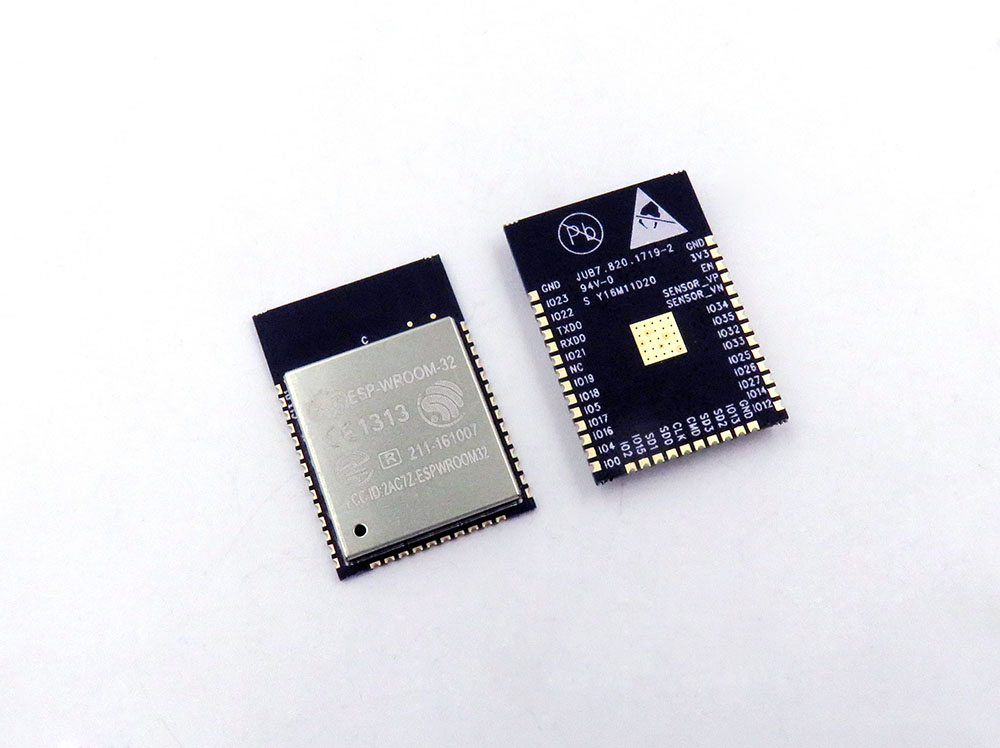
\includegraphics{Imagenes/esp32-wroom-s32-00}
\end{figure}

%http://www.electrodragon.com/product/wroom-32/


\subsection{Control de potencia AC por ángulo de fase}

%Curso práctico de Electrónica Inductrial y Automatización, CEKIT, Marzo 2001.


%TRIACS, detector de cruce por cero, optoacopladores
Los SCR y los TRIAC, permiten aplicar una técnica muy conveniente y eficaz para controlar el voltaje promedio y por lo tanto la potencia aplicada a una carga, cambiando el ángulo de fase con el cual la fuente de voltaje se aplica a ésta. Esta técnica de control de voltaje es muy usada en las aplicaciones de regulación de motores, iluminación y temperatura, por ser el voltaje la variable principal en estos tres procesos.\\

Para entender como se controla el ángulo de fase, por medio de un TRIAC conectado en serie con la carga, se puede asumir que el TRIAC se comporta idealmente como un interruptor controlador por la corriente de compuerta Ig que se cierra o se abre ante su presencia o ausencia. Observando la figura XX puede verse el control de una onda seno de tensión con un período con un período de 360 grados; en la parte (a) de la figura se muestra la tensión a través del TRIAC, mientras que en la parte (b) se ve la tensión sobre la carga; allí puede verse que el TRIAC se comporta como un circuito abierto durante los primero 45 grados de cada semiciclo, y todo el voltaje cae en sus terminales eliminando el flujo de corriente por la carga. La porción del semiciclo durante la cual se presenta esta situación se conoce como ángulo de disparo.\\

Una vez el TRIAC es disparado a través de su terminal de compuerta (G), éste se engancha y se comporta como un interruptor cerrado, permitiendo que todo el voltaje se aplique a la carga durante los 135 grados restantes de cada semiciclo. La porción del semiciclo durante la cual el TRIAC conduce se denomina ángulo de conducción.\\


\subsection{Control de Cargas DC}

%Switch y control de cargas DC PWM

\subsection{I2C}

\subsection{Sensores}

\subsubsection{Módulo GY-30}

Sensor GY-30 BH1750FVI. Es un sensor digital de intensidad de luz ambiente, tiene un conversor ADC de 16bits interno y comunicación por I2C. Esta es una versión mejorada del típico sensor de luz a base de un LDR, el cual simplemente entrega un valor analógico. Compatible con Arduino, PIC, etc. 

El módulo BH1750 es un sensor de luz, que a diferencia del LDR es digital y nos entrega valores de medición en Lux ( lumen /m$^2$ ) que es una  unidad de medida estándar para el nivel de iluminación (iluminancia). Tiene alta precisión y un rango ente 1 – 65535 lx el cual es configurable.

La interfaz de comunicación es I2C pudiéndolo implementar en la mayoría de micro controladores, el módulo aparte de los pines de alimentación y pines I2C tiene un pin para establecer la dirección.

%https://www.amgkits.com/home/113-sensor-de-intensidad-optica-sensor-de-luz-gy-30-bh1750fvi.html

\subsubsection{Temperatura y Humedad DHT11}

El DHT11 es un sensor de temperatura y humedad digital de bajo costo. Utiliza un sensor capacitivo de humedad y un termistor para medir el aire circundante, y muestra los datos mediante una señal digital en el pin de datos (no hay pines de entrada analógica). Es bastante simple de usar, pero requiere sincronización cuidadosa para tomar datos. El único inconveniente de este sensor es que sólo se puede obtener nuevos datos una vez cada 2 segundos, así que las lecturas que se pueden realizar serán mínimo cada 2 segundos.

%https://electronilab.co/tienda/sensor-de-temperatura-y-humedad-dht11/

\subsubsection{Módulo sensor de calidad de aire MQ-135}

Los sensores de gas de la serie MQ son sensores analógicos por lo que son fáciles de implementar con cualquier microcontrolador.

Estos sensores son electroquímicos y varían su resistencia cuando se exponen a determinados gases, internamente posee un calentador encargado de aumentar la temperatura interna y con esto el sensor pueda reaccionar con los gases provocando un cambio en el valor de la resistencia. El calentador dependiendo del modelo puede necesitar un voltaje entre 5 y 2 voltios, el sensor se comporta como una resistencia y necesita una resistencia de carga (RL) para cerrar el circuito y con este hacer un divisor de tención y poder leerlo desde un microcontrolador:

Debido al calentador es necesario esperar un tiempo de calentamiento para que la salida sea estable y tenga las características que el fabricante muestra en sus datasheet, dicho tiempo dependiendo del modelo puede ser entre 12 y 48 horas.

En el mercado, generalmente los sensores MQ se encuentran en módulos, lo que nos simplifica la parte de conexiones y nos facilitan su uso, solo basta con alimentar el módulo y empezar a leer el sensor, estos módulos también tienen una salida digital la cual internamente trabaja con un comparador y con la ayuda de un potenciómetro podemos calibrar el umbral y así poder interpretar la salida digital como presencia o ausencia del gas.

El Sensor Calidad Aire MQ135 se utilizan en equipos de control de calidad del aire para edificios y oficinas, son adecuados para la detección de NH3, NOx, alcohol, benceno, humo, CO2, etc.

Este sensor es sensible en similar proporción a los gases mencionados, con lo que podemos determinar si el aire está limpio.

%http://www.naylampmechatronics.com/blog/42_Tutorial-sensores-de-gas-MQ2-MQ3-MQ7-y-MQ13.html

Este sensor no proporciona valores absolutos, sino que simplemente proporciona una salida analógica que debe ser monitoreado y se comparada con los valores de umbral.
%http://www.geekbotelectronics.com/producto/mq-135-modulo-sensor-de-calidad-del-aire/

\subsubsection{Sensores de Estado}

Los sensores de estado describen si la variable esta en alto (1) o en bajo (0), para estos sensores se tienen diferentes variables tipicamente, como el estado de una puerta o una ventana (abierta o cerrada), la lluvia, el movimiento.

\paragraph{Módulo detector de lluvia: }
%http://panamahitek.com/modulo-yl-83-un-detector-de-lluvia/

\paragraph{Módulo PIR HC-SR501: }

https://puntoflotante.net/MODULO-SENSOR-PASIVO-INFRARROJO-PIR-HC-SR501.htm

http://www.naylampmechatronics.com/sensores-proximidad/55-modulo-de-deteccion-pir-hc-sr501.html

\subsection{Corriente Alterna (AC)}

\subsection{Corriente Directa (DC)}

\section{Software}

\subsection{RTOS}

\cite{SO} Los sistemas operativos en tiempo real, tienen como parámetro clave al tiempo, ya que en gran variedad de situaciones, como por ejemplo, un proceso industrial, se requiere recolectar múltiples datos, los cuales son usados para el control de múltiples procesos, los cuales deben ser ejecutados en determinados instantes, de no ser así, podría causar desde la mala ejecución de una tarea, hasta un accidente según la delicadeza del proceso.\\ 

Para procesos con nula tolerancia a fallos, se conoce como un sistema en tiempo real duro, muchos de estos sistemas se encuentran en el control de procesos industriales, en aeronáutica, en la milicia y en áreas de aplicación similares. el caso contrario, cuando se tiene cierta tolerancia a que muy ocasionalmente existan fallos, se conoce como sistema en tiempo real suave, los sistemas de audio digital o de multimedia están en esta categoría. Los teléfonos digitales también son ejemplos de sistema en tiempo real suave. \\


%Otro tipo de sistema operativo es el sistema en tiempo real. Estos sistemas se caracterizan por tener el tiempo como un parámetro clave. Por ejemplo, en los sistemas de control de procesos industriales, las computadoras en tiempo real tienen que recolectar datos acerca del proceso de producción y utilizarlos para controlar las máquinas en la fábrica. A menudo hay tiempos de entrega estrictos que se deben cumplir. Por ejemplo, si un auto se desplaza sobre una línea de ensamblaje, deben lle- varse a cabo ciertas acciones en determinados instantes. Si un robot soldador realiza su trabajo de soldadura antes o después de tiempo, el auto se arruinará. Si la acción debe ocurrir sin excepción en cierto momento (o dentro de cierto rango), tenemos un sistema en tiempo real duro. Muchos de estos sistemas se encuentran en el control de procesos industriales, en aeronáutica, en la milicia y en áreas de aplicación similares. Estos sistemas deben proveer garantías absolutas de que cierta acción ocurrirá en un instante determinado. 

%Otro tipo de sistema en tiempo real es el sistema en tiempo real suave, en el cual es acepta- ble que muy ocasionalmente se pueda fallar a un tiempo predeterminado. Los sistemas de audio di- gital o de multimedia están en esta categoría. Los teléfonos digitales también son ejemplos de sistema en tiempo real suave. 

``Como en los sistemas en tiempo real es crucial cumplir con tiempos predeterminados para realizar una acción, algunas veces el sistema operativo es simplemente una biblioteca enlazada con los programas de aplicación, en donde todo está acoplado en forma estrecha y no hay protección entre cada una de las partes del sistema. Un ejemplo de este tipo de sistema en tiempo real es freeRTOS.  Las categorías de sistemas para computadoras de bolsillo, sistemas integrados y sistemas en tiempo real se traslapan en forma considerable. Casi todos ellos tienen por lo menos ciertos aspectos de tiempo real suave. Los sistemas integrados y de tiempo real sólo ejecutan software que colocan los diseñadores del sistema; los usuarios no pueden agregar su propio software, lo cual facilita la protección. \\

Los sistemas de computadoras de bolsillo y los sistemas integrados están diseñados para los consumidores, mientras que los sistemas en tiempo real son más adecuados para el uso industrial. Sin embargo, tienen ciertas características en común''.\\

\subsection{ESP-IDF}

ESP-IDF es el entorno de desarrollo oficial para el ESP32 desarrollado por Espressif System, el cual mediante una serie de comandos específicos escritos en la terminal (para el caso de linux), permite realizar una configuración del ESP32 en cuanto a su funcionamiento, es decir, permite encender o apagar características como el WiFi, el Bluetooth o realizar particiones de memoria, ademas de esto, se puede cargar el código por el puerto USB al ESP32, al igual que se puede visualizar la información generada por el ESP32 por este mismo puerto.\\

\subsubsection{FreeRTOS}

%http://esp-idf.readthedocs.io/en/latest/api-reference/system/freertos.html

\subsubsection{Wi-Fi}

%http://esp-idf.readthedocs.io/en/latest/api-reference/wifi/esp_wifi.html

\subsubsection{Particiones}

%http://esp-idf.readthedocs.io/en/latest/api-guides/partition-tables.html

\subsubsection{Consola}

%http://esp-idf.readthedocs.io/en/latest/api-guides/console.html

\subsubsection{OTA}

%http://esp-idf.readthedocs.io/en/latest/api-reference/system/ota.html

\subsubsection{HTTP Request}
\subsubsection{Timers}

\subsection{Proteus}

